\documentclass[a4paper,12pt]{article}

\usepackage [utf8x] {inputenc} %кодировка исходного текста
\usepackage [T2A] {fontenc} %кодировка
\usepackage [english, russian] {babel}
\usepackage{color}
\usepackage{amsmath, amsfonts, amssymb, amsthm, mathtools}
\usepackage{graphicx}
\graphicspath{{.}}
\DeclareGraphicsExtensions{.pdf,.png,.jpg}
\righthyphenmin=2


\begin{document}

\title{Лабораторная работа №0: арифметика и основы работы с листингами}
\author{Дроздов Т. А. Б03-202}
\date{09.2023}

Написал стандартный  "Hello, world!" на плюсах, собрал программу и сгенерировал ассемблерный листинг. 

\begin{figure}[h] % так вставляются скриншоты с кодом и его выводом
	\centering
	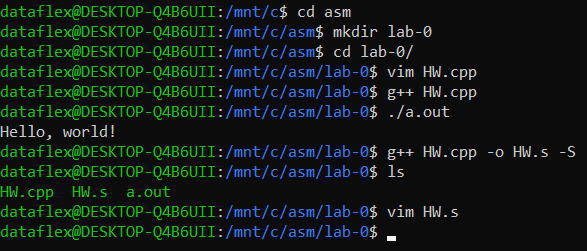
\includegraphics[width=0.8\linewidth]{command_line_asm.png}
\end{figure}


\begin{figure}[h] % так вставляются скриншоты с кодом и его выводом
	\centering
	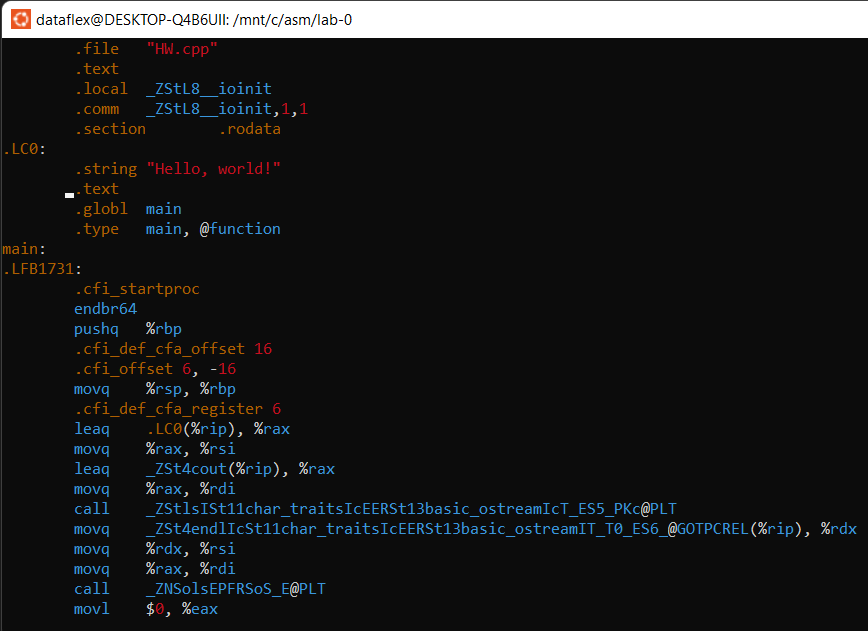
\includegraphics[width=0.8\linewidth]{HW s.png}
\end{figure}



Написал простейшую арифметическую программу, собрал, сгенерировал листинг. В листинге заменил команду addl на subl. Построил новый экзешник из листинга.


\begin{figure}[h] % так вставляются скриншоты с кодом и его выводом
	\centering
	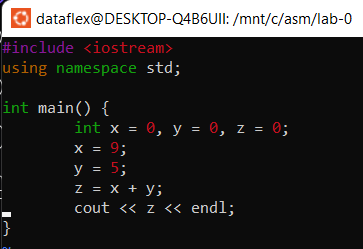
\includegraphics[width=0.8\linewidth]{arithmetic cpp.png}
\end{figure}


\begin{figure}[h] % так вставляются скриншоты с кодом и его выводом
	\centering
	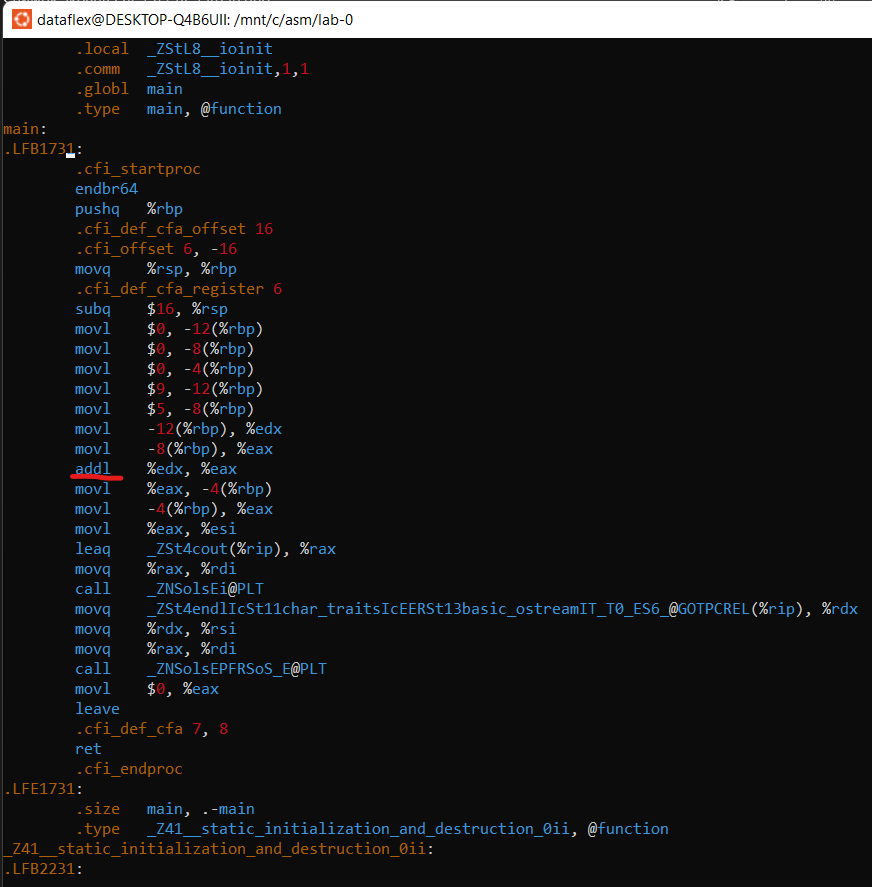
\includegraphics[width=0.8\linewidth]{arithmetic add.png}
\end{figure}


\begin{figure}[h] % так вставляются скриншоты с кодом и его выводом
	\centering
	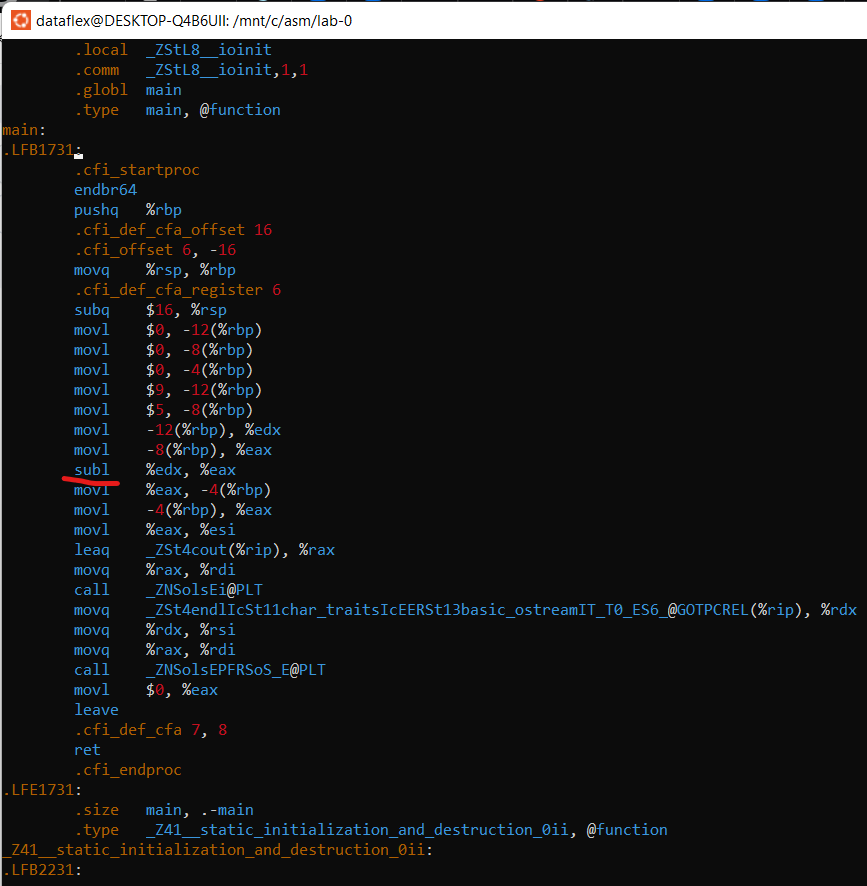
\includegraphics[width=0.8\linewidth]{arithmetic sub.png}
\end{figure}


\begin{figure}[h] % так вставляются скриншоты с кодом и его выводом
	\centering
	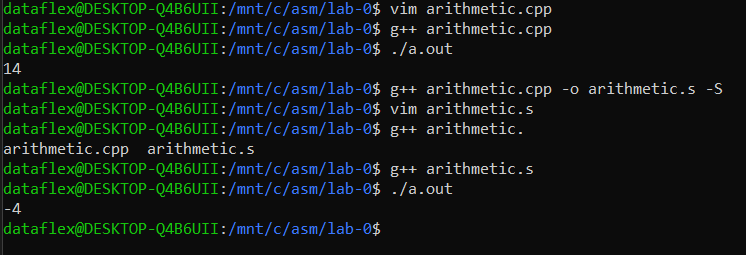
\includegraphics[width=0.8\linewidth]{arithmetic command line.png}
\end{figure}



\end{document}
